\documentclass[multi,tikz,crop=false,class=article]{standalone}

\onlyifstandalone{\usepackage{hyperref}
\usepackage{cleveref}
\usepackage[disable]{todonotes}
\presetkeys{todonotes}{inline, noline}{}
\usepackage{caption}
\usepackage{subcaption}
\usepackage{amsfonts}
\usepackage{theorem}
\usepackage{algorithm}
\usepackage{algpseudocode}
\theoremstyle{plain}
\theorembodyfont{\slshape}
\newtheorem{definition}{Definition}[section]
\usepackage{algorithm}
\usepackage{algpseudocode}
\usepackage{amsmath}
\usepackage{mathtools}
\usepackage{tikz}

\usetikzlibrary{automata,arrows}

%\DeclareCaptionType{algorithm}
\algdef{SE}[DOWHILE]{Do}{doWhile}{\algorithmicdo}[1]{\algorithmicwhile\ #1}%

% Math macros
\newcommand{\concat}{\cdot}
\newcommand{\bool}{\ensuremath{\mathbb{B}}}
\newcommand{\lang}{\ensuremath{\mathcal{L}}}
\newcommand{\dstar}[2]{\ensuremath{\delta^*(#1,#2)}}
\newcommand{\exec}[2]{\ensuremath{#1[#2]}}
\newcommand{\access}[2]{\ensuremath{#1^{-1}[#2]}}
\newcommand{\nero}{\ensuremath{\equiv}}
\newcommand{\eqclass}[2]{\ensuremath{[#1]_{#2}}}
\newcommand{\mq}{\ensuremath{\mathsf{member}}}
\newcommand{\eq}{\ensuremath{\mathsf{equiv}}}
\newcommand{\row}{\ensuremath{\mathsf{row}}}
\newcommand{\sift}{\ensuremath{\mathsf{sift}}}
%%% Local Variables:
%%% mode: latex
%%% TeX-master: t
%%% End:
}
\usetikzlibrary{automata,arrows}

\begin{document}
\section{Variants}
\label{sec:variants}
In the first few years following the introduction of the L* algorithm by
D. Angluin~\cite{Angluin87}, L* learning was only a theoretical exploration.
The various improvements described in the previous chapter,
such as \textit{Classification Trees} \cref{sec:classification-trees} and
the \textit{TTT} algorithm \cref{sec:ttt}
made practical applications already more feasible.

In applying L* or improvements thereof to practical applications,
there were still some practical limitations and restrictions that had to
be addressed (Steffen 2011, Ch. 6~\cite{Steffen11}).
Some of these issues can be summarized as follows:
\begin{itemize}
  \item Equivalence queries are generally undecidable for black boxes
  \item L* can only interact with regular languages, not with real systems
  \item The amount of required membership queries can grow very fast
  \item Membership queries might not be independent in practice,
        which imposes the requirement for a \textit{reset} function
  \item Not all systems might support a \textit{reset} function.
\end{itemize}

In order to address these limitations and restrictions,
several variants of the L* algorithm have been proposed,
each with the goal to solve such an issue.
In this chapter we will further elaborate on some of these issues
and the variants proposed to solve them.

\subsection{Approximating \textit{EQUIV (M)} queries with \textit{MEMBER (w)} queries}
The target machine on which the learning algorithm is applied is generally
a black box, since the main motive for using a learning algorithm is to
infer knowledge about some unknown system.
Therefore equivalence queries can generally only be answered by exhaustively
testing the inputs and outputs of a system.
However, exhaustively testing a black box is undecidably hard.

In order to solve this issue model-based testing techniques have been used,
such as \textit{Chow's W-method} or the \textit{WP-method} \todo{Cite here}.
These methods rely on approximating \textit{EQUIV (M)} queries by using
\textit{MEMBER (w)} queries.

To further research in this area,
the \textit{ZULU} challenge~\cite{Combe10} was introduced.
The \textit{ZULU} challenge asked participants to find a DFA corresponding
to a certain system as accurately as possible, while imposing a restriction
on the number of \textit{MEMBER (w)} queries and disallowing \textit{EQUIV (M)}
queries completely.
\todo{Elaborate on ZULU some more}

\subsection{Limiting the amount of membership queries}
In a theoretical framework the learning algorithm doesn't have to account
for execution times of individual \textit{MEMBER (w)} queries.
In practice, such queries might take time or be expensive to execute.
Therefore algorithms benefit from reducing the amount of queries needed.
Some generic improvements in this regard have already been covered in
\todo{Reference previous chapter}.

However, when using for example \textit{Chow's method} for \textit{EQUIV (M)}
queries, the amount of membership queries needed grows exponentially
in the number of states \todo{Cite source for exponential complexity of Chow's}.

\todo{Cite ZULU participant here, since the challenge also imposed
      a maximum on \textit{MEMBER (w)} queries}

\subsection{Learning Mealy machines}
The $L^*$ algorithm of Angluin is able to learn DFA's, but it can not directly learn mealy machines. A mealy machine, as opposed to a DFA, has no accepting states. Instead, mealy machines additionally define an output symbol on each state transition. Reactive systems, or I/O programs, are easily modeled by a mealy machine, but not as easily by a DFA. Therefore, some adaptations are required. There are two main ways to do this. Either the mealy machine can be transformed into a DFA, or an adaptation of $L^*$ called $L^*_{M}$ can be used to learn the mealy machine directly.

\subsubsection {Transforming a mealy machines into a DFA}
Say we have a mealy automaton $M$ with input alphabet $\Sigma_M$ and output alphabet $O$ that we want to transform into a DFA $D$ with input alphabet $\Sigma_D$. There are two ways to do this.

The first first way is define $\Sigma_D = \Sigma_M \cup O$ \cite{Hungar03}. This transformation defines that each state in $M$ is also a state in $D$. For each transition in $M$ from state $q_a$ to $q_b$ constrained by $i$ and output symbol $o$, a new intermediate state $q_t$ is introduced in $D$. Two transitions are added: one from $q_a$ to $q_t$ constrained by $i$, and one from $q_t$ to $q_b$ constrained by $o$. Furthermore, a single error state $k$ is added to $D$, which is the only non-accepting state. For each combination of a node $q$ and input symbol $\sigma \in \Sigma_D$, if $q$ does not yet contain a transition constrained by $\sigma$, a transition constrained by $\sigma$ is added from $q$ to $k$. An example of this transformation can be seen in figure \ref{fig:transformation_hungar}.

The second way to transform $M$ is to define $\Sigma_D = \Sigma_M \times O$ \cite{Makinen01}. In other words, $\Sigma_D$ contains all combinations of input and output symbols from $M$. This removes the need for intermediate states, but can have a significant impact on the size of the input alphabet. Similarly to the previous transformation, one error state is defined and all other states are accepting states. If from a certain state an input/output combination does not occur, then a transition to the error state is added with that combination. An example of this transformation can be seen in figure \ref{fig:transformation_makinen}.

Either of these transformations can be used to learn a mealy machine with the standard $L^*$ algorithm. \todo {for both of these, explain how membership queries are defined} To learn a mealy machine $M$, simply define $\Sigma$ as $\Sigma_M \cup O$ or $\Sigma_M \times O$. By doing this, a model $D$ is learned which is the transformed version of $M$.

\begin{figure}[t]
\centering
\begin{subfigure}[b]{.2\textwidth}
\centering
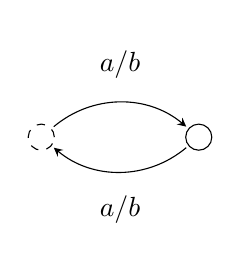
\begin{tikzpicture}
  [bend angle=40,every node/.style={draw,circle}]

  \tikzstyle{initial} = [dashed]

  \node[initial]   (1) at (1,0) {};
  \node 		   (2) at (3,0) {};

  \path[->, >=stealth, shorten > = 1pt, shorten < = 1pt]
        (1) edge [bend left] node[auto,draw=none] {$a/b$} (2) 
        (2) edge [bend left] node[auto,draw=none] {$a/b$} (1);
\end{tikzpicture}
\caption{Mealy representation} \label{fig:transformation_mealy}
\end{subfigure}
\hfill
\begin{subfigure}[b]{0.4\textwidth}
\centering
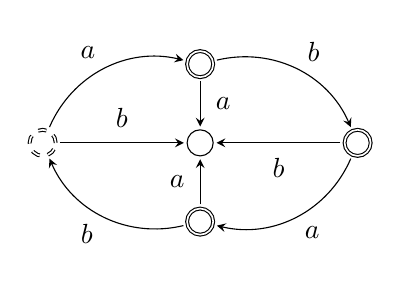
\begin{tikzpicture}
  [bend angle=40,every node/.style={draw,circle}]

  \tikzstyle{initial} = [dashed]

  \node[initial, accepting] (1) at (1,0)  {};
  \node 					(2) at (3,0)  {};
  \node [accepting] 		(3) at (5,0)  {};
  \node [accepting] 		(4) at (3,-1) {};
  \node [accepting] 		(5) at (3,1)  {};

  \path[->, >=stealth, shorten > = 1pt, shorten < = 1pt]
        (1) edge [bend left] node[auto,draw=none] {$a$} (5) 
        (4) edge [bend left] node[auto,draw=none] {$b$} (1)
        (5) edge [bend left] node[auto,draw=none] {$b$} (3)
        (3) edge [bend left] node[auto,draw=none] {$a$} (4)
        (1) edge 			 node[auto,draw=none] {$b$} (2)
        (3) edge 			 node[auto,draw=none] {$b$} (2)
        (4) edge 			 node[auto,draw=none] {$a$} (2)
        (5) edge 			 node[auto,draw=none] {$a$} (2);
\end{tikzpicture}
\caption{Hungar's transformation} \label{fig:transformation_hungar}
\end{subfigure}
\centering
\begin{subfigure}[b]{.3\textwidth}
\centering
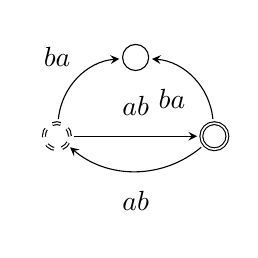
\begin{tikzpicture}
  [bend angle=40,every node/.style={draw,circle}]

  \tikzstyle{initial} = [dashed]

  \node[initial, accepting]   (1) at (1,0) {};
  \node[accepting] (2) at (3,0) {};
  \node (3) at (2,1) {};

  \path[->, >=stealth, shorten > = 1pt, shorten < = 1pt]
        (1) edge 			  node[auto,draw=none] {$ab$} (2) 
        (2) edge [bend left]  node[auto,draw=none] {$ab$} (1)
        (1) edge [bend left]  node[auto,draw=none] {$ba$} (3)
        (2) edge [bend right] node[auto,draw=none] {$ba$} (3);
\end{tikzpicture}
\caption{M\"{a}kinen's transformation} \label{fig:transformation_makinen}
\end{subfigure}
\caption{Mealy to DFA transformation} \label{fig:transformation}
\end{figure}

\subsubsection {Adapting $L^*$ into $L^*_{M}$}

Adapting Angluin's $L^*$ algorithm has been adjusted for use with mealy machines. The new procedure was first informally described in \cite{Margaria04}, and later more rigorously in \cite{Shahbaz09}. In $L^*$ the membership queries return a boolean value; either it's a member, or it's not. For $L^*_{M}$, the membership query is replaced by a output query, which returns an output string. The observation table is modified to store these output strings instead of boolean values. As in $L^*$, output queries are used in order to fill in the observation table. Suppose the algorithm performs an output query for $s \concat e$, where $s \in S \cup (S \concat \Sigma)$ and $e \in E$. The query will produce a string $r$ with $|r| = |s| + |e|$, where $|x|$ denotes the length of the string x. Instead of storing $r$ directly in the observation table, only the last $|e|$ symbols of $r$ are stored (since the observation is prefix closed, the output corresponding to $s$ is already stored in the table). The intuitive meaning of this value is that it corresponds to the sequence of output symbols that is produced when the when input $e$ is applied from the state corresponding to $s$. 

With the new meaning of the values in the table, a value of $\epsilon$ in $E$ becomes nonsensical. This is because $\epsilon$ would denote no change in state, so there would be no output symbol. Therefore, at the start of the algorithm, $E$ is not intialized to $\{\epsilon\}$ but to $\Sigma$. 

The concepts of closedness and consistency remain identical. The procedure to build the hypothesis remains largely the same, but now the generated hypothesis no longer defines accepting states, but instead defines output strings on the transitions.
\todo {note that mealy ≃ dfa}

\subsection{Systems without a \textit{reset} function}
\label{sec:noreset}
In the L* learning algorithm, every \textit{MEMBER (w)} query is implicitly
independent of other queries.
However, when learning a system in practice, it might happen that
\textit{MEMBER (w)} queries are not independent at all.
Suppose for example that the system under learning requires authentication
while also imposing a restriction on the maximum amount of failed requests.
In such a system queries are no longer independent of each other,
since after a certain amount of authentication requests
the systems behaviour suddenly changes for the same membership queries.
In order to solve this issue, the L* algorithm implicitly requires a means
of \textit{reset}ting the system under learning (Rivest \& Schapire, pg. 301)\cite{Rivest93}.

However, not all systems support a \textit{reset} function.
As we'll see in \todo{reference applications}, the system under learning
could also be a system that the learning algorithm has totally no control over.

\subsection{}

\end{document}

%%% Local Variables:
%%% mode: latex
%%% TeX-master: "main"
%%% End:
